\Chapter{Introduction}
\label{chap:introduction}

\mode<article>{
This course is focused on the subject of computer networks.
It is safe to presume that all participants have a basic understanding of what a computer is, despite the fact that many devices contain a computer without the user being aware of it.
For example, the \abbr{ATM}%
   \footnote{Here \abbr{ATM} stands for automated teller machine; in the rest of the notes it stands for \acl{ATM}.}
used to withdraw money from a bank account, the computer systems present in modern vehicles, and even studio mixers%
   \footnote{For example, \href{https://www.presonus.com/learn/technical-articles/How-To-Network-Studiolive-Digital-Mixers-for-Remote-Control}{this article} explains how to connect a PreSonus StudioLive 16 to the network for remote control. But it is also possible to send the audio over the network to the mixer.}
, which often feature a network interface, are all examples of computers.
% Dante for AV systems: https://www.audinate.com/meet-dante/what-is-dante
% Art-Net for lighting systems: https://art-net.org.uk
    
When you connect these computers together using network cables or using wireless network adapters, they form a network.
A computer network is used to exchange information between different computers.

In this introductory chapter we will first discuss a few names used to talk about the geographic and organisational size of a network.
We will then take a look at some different topologies that can arise when connecting computers together in a network.
This includes both physical and logical topologies.

Next we will take a look at the history and evolution of computer networks and we differentiate between 
local networks and wide-area networks, of which the internet is the best-known example.

We then move on to a more theoretical part of the introduction where we will talk about the networking models and explain what a protocol is, as well as give some examples.
We also cover routing schemes.
We will ask some questions about how network communication goes and circle back to the network models when we talk about encapsulation.
Finally, we will talk about network symbols used in literature to create network diagrams.




\section{Network size}
\label{sec:network-size}

Networks may be characterised by many properties or features, such as physical capacity, organisational scope (\vref{sec:network-ownership}), user authorisation, access rights, and others.
Another distinct classification method is that of the physical extent or geographic scale.

\paragraph{\gls{LAN}}\iacs{LAN}
A computer network that interconnects computers within a limited area such as a residence, school, laboratory, or office building.

The term \gls{LAN} can be used both for a single \emph{broadcast domain} (see \vref{sec:routing-schemes,sec:routing}) or local network, similar to a \acs{WLAN} being a single wireless broadcast domain and a `\acs{VLAN}' being a virtual \gls{LAN} defined on a switch or group of switches; but the term `\gls{LAN}' can also mean the group of all of these local networks, forming the complete company or home network.
In that case, `local' refers to the geographic location (one building) instead of the physical property of the network (a single broadcast domain).

\paragraph{\gls{WAN}}\iacs{WAN}
   \index{telecommunication circuit}
   \index{leased line}
A telecommunications network that extends over a large geographic area.
Wide-area networks are often established with \emph{leased telecommunication circuits}.
These networks are mostly operated by \glspl{ISP}.

\paragraph{\gls{PAN}}\iacs{PAN}
A computer network for interconnecting electronic devices within an individual person's workspace.
One example is your mobile phone pairing wirelessly with your watch and ear buds.

\paragraph{\gls{CAN}}\iacs{CAN}
A computer network made up of an interconnection of local-area networks within a limited geographical area.
The networking equipment (switches, routers) and transmission media (optical fibre, copper plant, cat~5 cabling, etc.) are almost entirely owned by the campus tenant or owner: an enterprise, university, government, etc.
A \acl{CAN} is larger than a \acl{LAN} but smaller than a \acs{MAN} or \gls{WAN}.

An example would be the High Tech Campus in Eindhoven.\index{High Tech Campus}
The buildings house different companies which are all interconnected using fibre optic cabling owned and maintained by the campus' \acs{IT} team.
The campus also has its own data centres and provides redundant connections to the internet.

\paragraph{\gls{MAN}}%
   \iacs{MAN}
A computer network that interconnects users with computer resources in a geographic region of the size of a metropolitan area.
The term \gls{MAN} is applied to the interconnection of local-area networks in a city into a single larger network which may then also offer efficient connection to a wide-area network.

\paragraph{\gls{SAN}}%
   \iacs{SAN}
A computer network which provides access to consolidated, block-level data storage.
\glspl{SAN} are primarily used to access data storage devices, such as disk arrays and tape libraries from servers so that the devices appear to the operating system as direct-attached storage.
A \gls{SAN} typically is a dedicated network of storage devices not accessible through the local-area network.
\Gls{NAS} is file-level storage such as Windows file shares using the \acs{SMB} protocol and is thus not the same as a \acs{SAN}.
\iacs{NAS}




\section{Network ownership}
\label{sec:network-ownership}

\paragraph{internet}%
   \index{internet}
   \index{internetwork}
An internetwork is the connection of multiple different computer networks to form a single network.

The internet is the largest example of an internetwork.
It is a global system of interconnected governmental, academic, corporate, public, and private computer networks.
Participants on the internet use a diverse array of methods of several hundred documented, and often standardised, protocols compatible with the \acl{IP} suite and an addressing system (\acs{IP} addresses).
Service providers and large enterprises exchange information about the reachability of their address spaces through the \acf{BGP}\iacs{BGP} (see \vref{sec:routing}), forming a redundant worldwide mesh of transmission paths.

\paragraph{intranet}\index{intranet}
An intranet is a set of networks that are under the control of a single administrative entity.
The intranet uses the \gls{IP} and \gls{IP}-based tools such as web browsers and file transfer applications.
The administrative entity limits the use of the intranet to its authorised users.
Most commonly, an intranet is the internal \gls{LAN} of an organisation.
A large intranet typically has at least one web server to provide users with organisational information.
An intranet is also anything behind the router on a local-area network.

\paragraph{extranet}\index{extranet}
An extranet is a network that is also under the administrative control of a single organisation but supports a limited connection to a specific external network.
For example, an organisation may provide access to some aspects of its intranet to share data with its business partners or customers.
These other entities are not necessarily trusted from a security standpoint.
Network connection to an extranet is often, but not always, implemented via \gls{WAN} technology, such as IPsec \acs{VPN} tunnels.\index{VPN@\acs{VPN}!IPsec}

\paragraph{\gls{DMZ}}\iacs{DMZ}
A \gls{DMZ} is similar to an extranet but where an extranet only provides access to resources for a limited subnet of business partners or customers, services hosted in a \gls{DMZ} are generally accessible by anyone on the internet.
It is an isolated and heavily firewalled part of a company's intranet.


\Section{Network topologies}
\label{sec:network-topologies}

\mode<article>{
The network \emph{topology} is the arrangement of the elements (links, nodes, etc.) of a communication network.
It can be used to define or describe the arrangement of various types of telecommunication networks, including computer networks.

Network topology is the topological structure of a network and may be depicted physically or logically.
The physical topology describes how the components are physically connected together, while the logical topology illustrates how data flows within a network.
Distances between nodes, physical interconnections, transmission rates, or signal types may differ between two different networks, yet their logical topologies may be identical.
A network’s physical topology is a particular concern of the physical layer of the \gls{OSI} model (\vref{sec:network-models}).
}


\Paragraph{point-to-point}
\mode<article>{
The simplest method of connecting two devices together in a network is to directly connect them together using a cable for transfering data.
This could be a network cable but can also be a serial or parallel cable.
}

\Paragraph{ring}
\mode<article>{
   \index{topology (network)!ring}
Each node connects to exactly two other nodes, forming a single continuous pathway for signals through each node -- a ring.
Data travels from node to node, with each node along the way handling every packet.

Token Ring is an example of a \gls{LAN} technology that uses a logical ring topology.
The physical topology of a Token Ring network is a star as the devices are interconnected using a \ac{MAU}, a device similar to an Ethernet network switch.
The Telenet backbone is an example of interconnecting physical ring structures though the logical structure is a mesh of point-to-point links.
}

\Paragraph{bus}
\mode<article>{
   \index{topology (network)!bus}
Nodes are directly connected to a common \emph{half-duplex}%
   \index{half duplex}%
\footnote{A half-duplex (\abbr{HDX}) system provides communication in both directions, but only one direction at a time, not simultaneously in both directions.}
link called a bus.
An example of a physical bus structure, would be the old Ethernet networks using coaxial cable.
Connecting devices together using cat.~5-cable and a hub, results in a logical bus structure even though the physical structure is a star.
}

\Paragraph{star}
\mode<article>{
   \index{topology (network)!star}
Every host is connected to a central hub.
In its simplest form, one central hub acts as a conduit to transmit messages.
The star network is one of the most common computer network topologies.
}

\Paragraph{mesh}
\mode<article>{
   \index{topology (network)!mesh}
The infrastructure nodes connect directly, dynamically and non-hi\-er\-ar\-chi\-cal\-ly to as many other nodes as possible and cooperate with one another to efficiently route data to and from clients.
A \emph{full} mesh is a network where every node has a connection to every other node.
A \emph{partial} mesh is a network where some of the connects of a full mesh are missing.
}



\section{Network evolution}
\label{sec:network-evolution}

Let's briefly examine the evolution of both local-area networks and wide-area networks.

\subsection{Local-area networks}
\label{sec:network-evolution-lan}

\paragraph{mainframe (1970)}%
   \index{mainframe}
By the early 1970s, many mainframes acquired interactive user terminals operating as time-sharing computers, supporting hundreds of users simultaneously along with batch processing.
Users gained access through keyboard or typewriter terminals%
   \index{terminal}
and specialised text terminal \gls{CRT} displays with integral keyboards, or later from personal computers equipped with terminal emulation software.

These terminals used proprietary cabling.
Replacing your mainframe with a model from a competitor thus also meant replacing all cables in the walls.
    
\paragraph{\acl{SNA} (1974)}
\Gls{SNA} is IBM's proprietary networking architecture, created in 1974.
It is a complete protocol stack for interconnecting computers and their resources.
\gls{SNA} describes formats and protocols and is, in itself, not a piece of software.
The implementation of \gls{SNA} takes the form of various communications packages, most notably \gls{VTAM}, the mainframe software package for \gls{SNA} communications.
    
\paragraph{thicknet (1980)}%
   \index{thicknet}%
   \index{10BASE5@\abbr{10BASE5}}%
   \index{Ethernet!thick}%
   \index{coaxial cable}
% https://en.wikipedia.org/wiki/10BASE5
\abbr{10BASE5} (also known as thick Ethernet or \emph{thicknet}) was the first commercially available variant of Ethernet.
The technology was standardised in 1982 as \acs{IEEE} 802.3.
\abbr{10BASE5} uses a thick and stiff coaxial cable up to 500~metres in length.
Up to 100~stations can be connected to the cable using vampire taps and share a single collision domain with \SI{10}{\mega\bit\per\second}%
   \footnote{These units are often displayed as `Mbps' for megabit-per-second. In this case it is important to differentiate between a lowercase `b' for bit and an uppercase `B' for byte.}
of bandwidth shared among them.
The system is difficult to install and maintain.

\paragraph{Token Ring (1984)}%
   \index{Token Ring}%
   \index{token}
Token Ring is a computer networking technology used to build local-area networks.
It was introduced by IBM in 1984, and standardised in 1989 as \acs{IEEE} 802.5.

It uses a special three-byte frame called a \emph{token} that is passed around a logical ring of workstations or servers.
This token passing is a channel access method providing fair access for all stations, and eliminating the collisions of contention-based access methods.

Token Ring was a successful technology, particularly in corporate environments, but was gradually eclipsed by the later versions of Ethernet.

\paragraph{thinnet (1985)}%
   \index{thinnet}%
   \index{10BASE2@\abbr{10BASE2}}%
   \index{Ethernet!thin}%
   \index{coaxial cable}%
   \index{connectors!BNC@\acs{BNC}}
\abbr{10BASE2} (also known as cheapernet, thin Ethernet, \emph{thinnet}, and \emph{thinwire}) is a variant of Ethernet that uses thin coaxial cable terminated with \acs{BNC} connectors to build a local-area network.

During the mid to late 1980s this was the dominant \SI{10}{\mega\bit\per\second} Ethernet standard, but due to the immense demand for high speed networking, the low cost of \mbox{category-5} cable, and the popularity of 802.11 wireless networks, both \abbr{10BASE2} and \abbr{10BASE5} have become increasingly obsolete.

\paragraph{Ethernet switches (1985)}%
   \index{switch (Ethernet)}%
   \index{bridge (Ethernet)}%
   \index{Kempf, Mark}%
   \index{collision domain}
% https://en.wikipedia.org/wiki/Network_switch
Ethernet switches are the most common form of network switch.
The first \acs{MAC} bridge was invented in 1983 by Mark Kempf, an engineer in the Networking Advanced Development group of \gls{DEC}.
The first two-port bridge product (LANBridge 100) was introduced by that company shortly after.
The company subsequently produced multi-port switches for both Ethernet and \acs{FDDI} such as GigaSwitch.
Digital decided to license its \acs{MAC} bridge patent in a royalty-free, non-dis\-crim\-i\-na\-tory basis that allowed \acs{IEEE} standardisation.
This permitted a number of other companies to produce multi-port switches, including Kalpana.
Ethernet was initially a shared-access medium, but the introduction of the \acs{MAC} bridge began its transformation into its most-common point-to-point form without a collision domain.
Switches also exist for other types of networks including Fibre Channel, \gls{ATM}, and InfiniBand.
    
\subsection{Wide-area networks}
\label{sec:network-evoluation-wan}

\paragraph{ARPAnet (1971)}%
   \index{ARPAnet}%
   \index{Telnet}%
   \iacs{FTP}%
   \index{PDP-11@\abbr{PDP-11}}%
   \index{router}
The ARPAnet or Advanced Research Projects Agency network was the first wide-area packet-switched network with distributed control and one of the first networks to implement the \acs{TCP}/\acs{IP} protocol suite.
Both technologies became the technical foundation of the internet.
The first four nodes were designated as a testbed for developing and debugging the 1822 protocol, which was a major undertaking.
While they were connected electronically in 1969, network applications were not possible until the \gls{NCP}%
   \footnote{\acs{NCP} is the predecessor to \acs{TCP}.}
was implemented in 1970 enabling the first two host-to-host protocols, remote login (Telnet) and file transfer (\acs{FTP}) which were specified and implemented between 1969 and 1973.
The network was declared operational in 1971.
Network traffic began to grow once email was established at the majority of sites by around 1973.

Many of the earliest systems on the ARPAnet were \abbr{PDP-11}s, see \vref{fig:thompson}.%
\footnote{\href{https://www.truecable.com/blogs/cable-academy/a-brief-history-of-network-technology}{https://www.truecable.com/blogs/cable-academy/a-brief-history-of-network-technology}}
The \abbr{DECSA} communications server was a communications platform developed by \gls{DEC} based on a \abbr{PDP-11/24}, with the provision for user installable \gls{IO} cards including asynchronous and synchronous modules.
This product was used as one of the earliest commercial platforms upon which networking products could be built, including \abbr{X.25} gateways, \gls{SNA} gateways, routers, and terminal servers.%
\footnote{A terminal server connects devices with a serial port to a local-area network.}
Ethernet adapters were also available.

\begin{figure}
\centering
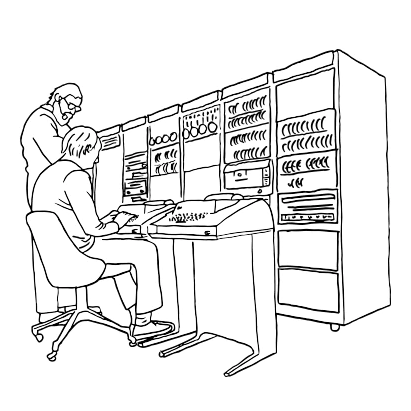
\includegraphics[width=.5\textwidth]{images/thompson.png}
\caption%
   [Thompson and Ritchie working on a \abbr{PDP-11}]%
   {Ken Thompson (sitting) and Dennis Ritchie working on a \abbr{PDP-11}, circa~1970. The picture was taken by Peter Hamer and the line drawing was made by \href{https://www.truecable.com/blogs/cable-academy/a-brief-history-of-network-technology}{truecable.com}.}
\label{fig:thompson}
\end{figure}

\paragraph{\abbr{X.25} (1976)}%
   \index{X.25@\abbr{X.25}}
\abbr{X.25} is an \acs{ITU-T} standard protocol suite for packet-switched data communication in \aclp{WAN}.
Is is one of the oldest packet-switching communication protocols available; it was developed several years before \gls{IP} version~4 (1981) and the \gls{OSI} reference model (1984).
The protocol suite is designed as three conceptual layers, which correspond closely to the lower three layers of the seven-layer \gls{OSI} model.
It also supports functionality not found in the \gls{OSI} network layer.
% TODO: such as?
% Perhaps "The X.25 data link layer, LAPB, provides a reliable data path across a data link (or multiple parallel data links, multilink) which may not be reliable itself." (wikipedia)

\paragraph{Minitel (1984)}
   \index{Minitel}%
   \index{terminal}%
   \index{modem}
In the early 1980s the French launched the Minitel project, an ambitious plan to bring data networking into everyone’s home.
Sponsored by the French government, the Minitel system consisted of a public packet-switched network, Minitel servers, and inexpensive terminals with built-in low-speed modems.
The Minitel became a huge success in 1984 when the French government gave away a free Minitel terminal to each French household that wanted one.
Minitel sites included free sites -- such as a telephone directory site -- as well as private sites, which collected a usage-based fee from each user.
At its peak in the mid 1990s, it offered more than twenty thousand services, ranging from home banking to specialised research databases.
The Minitel was in a large proportion of French homes ten years before most Americans had ever heard of the internet.

\paragraph{NSFnet (1985)}%
   \index{NSFnet}%
   \index{backbone (network)}
The National Science Foundation network (NSFnet) was a program of coordinated, evolving projects sponsored by the \gls{NSF} from 1985 to 1995 to promote advanced research and education networking in the United States.
The program created several nationwide backbone computer networks in support of these initiatives.
Initially created to link researchers to the \gls{NSF}-funded supercomputing centers, through further public funding and private industry partnerships it developed into a major part of the internet backbone.

The \acl{NSF} permitted only government agencies and universities to use the network until 1989 when the first commercial \acl{ISP} emerged.
By 1991, the \acs{NSF} removed access restrictions and the commercial \acs{ISP} business grew rapidly.

\paragraph{internet (1991)}%
   \index{internet}%
   \iacs{ISP}%
   \iacs{IXP}%
   \iacs{CDN}
The internet is a network interconnecting other networks in a partial mesh topology.
It consists of many \aclp{ISP}, \glspl{IXP}, \glspl{CDN}, companies, and other organisations.

\paragraph{IPsec virtual private networks (1995)}%
   \index{VPN@\acs{VPN}!IPsec}%
   \index{VPN@\acs{VPN}!MPLS@\acs{MPLS}}%
\Glspl{VPN} are private networks that run on top of a public network, either the internet in case of IPsec \gls{VPN} or the backbone of a service provider in case of \acs{MPLS} \gls{VPN}.
IPsec is used to encrypt the data sent over these virtual connections or tunnels and ensure confidentiality and integrity.

%\paragraph{MPLS virtual private networks (1999)}

\paragraph{cloud computing (2002)}%
   \index{cloud computing}
In July 2002, Amazon created subsidiary Amazon Web Services, with the goal to `enable developers to build innovative and entrepreneurial applications on their own.'
In March 2006 Amazon introduced its Simple Storage Service (\abbr{S3}), followed by Elastic Compute Cloud (\abbr{EC2}) in August of the same year.
These products pioneered the usage of server virtualisation to deliver IaaS at a cheaper and on-demand pricing basis.

\paragraph{YouTube (2005)}
Google launched YouTube on February 14, 2005 and was the beginning of ubiquitous video and massive amounts of user-generated content.


}


\Section{Routing schemes}
\label{sec:routing-schemes}
\mode<article>{
Routing schemes differ in how they deliver messages.
Unicast is the dominant form of message delivery on the internet.
}

\Paragraph{unicast}
\mode<article>{
   \index{routing scheme!unicast}
Unicast is a one-to-one transmission from one point in the network to another point (\cref{fig:unicast}); that is, one sender and one receiver, each identified by a network address.

\begin{figure}
\begin{minipage}{.4\textwidth}
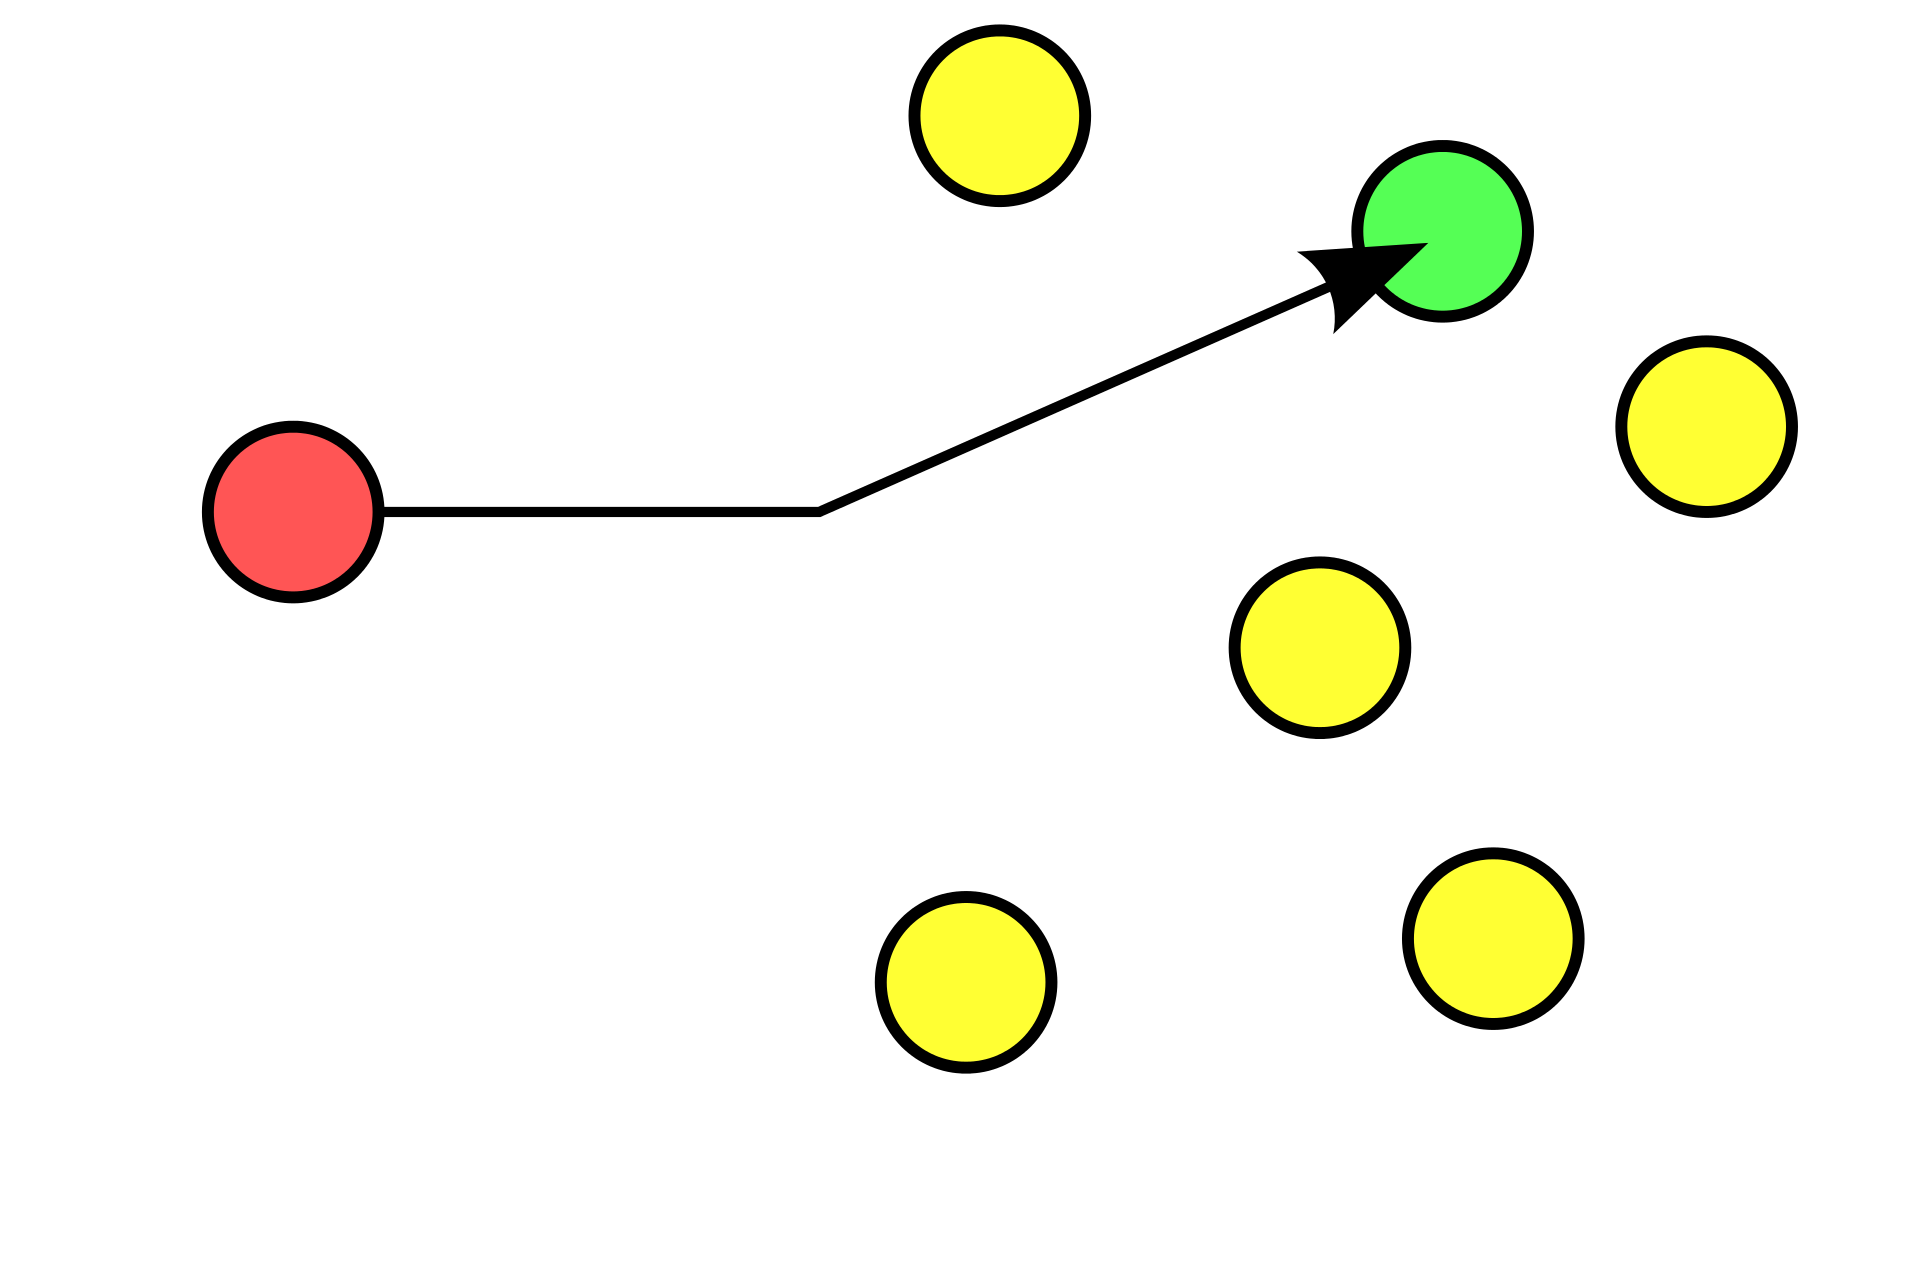
\includegraphics[width=\textwidth]{images/unicast.png}
\caption[Unicast routing scheme]{Unicast routing}
\label{fig:unicast}
\end{minipage}
\hfill
\begin{minipage}{.4\textwidth}
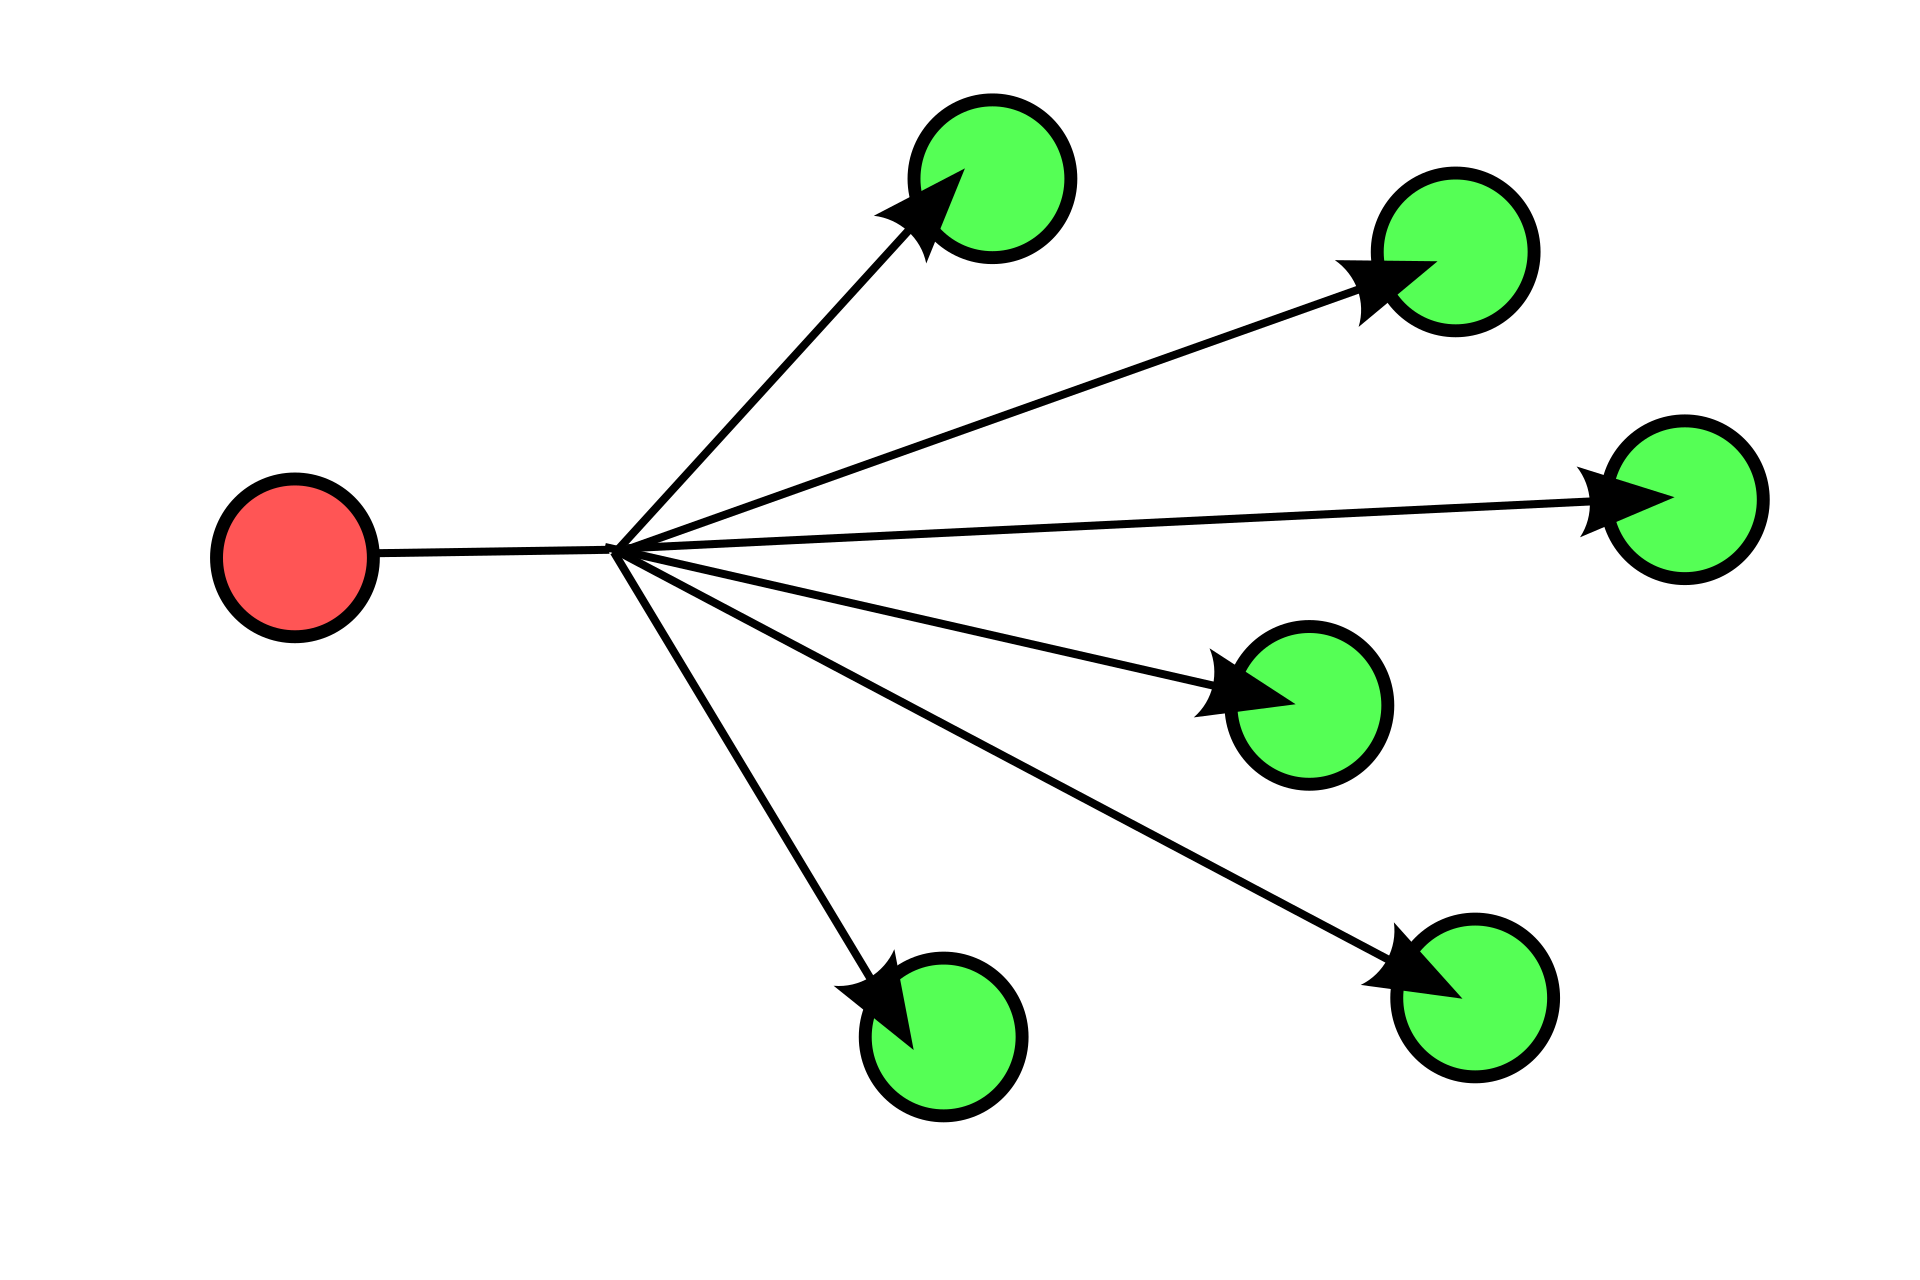
\includegraphics[width=\textwidth]{images/broadcast.png}
\caption[Broadcast routing scheme]{Broadcast routing}
\label{fig:broadcast}
\end{minipage}
\end{figure}
}

\Paragraph{broadcast}
\mode<article>{
   \index{routing scheme!broadcast}
Broadcasting is a method of transferring a message to all recipients simultaneously (\cref{fig:broadcast}).
Broadcasting can be performed as a high-level operation in a program, or it may be a low-level networking operation, for example broadcasting on Ethernet.
}

\Paragraph{multicast}
\mode<article>{
   \index{routing scheme!multicast}
Multicast is group communication where data transmission is addressed to a group of destination computers simultaneously (\cref{fig:multicast}).
Multicast can be one-to-many or many-to-many distribution.
}

\Paragraph{anycast}
\mode<article>{
   \index{routing scheme!anycast}
   \iacs{CDN}
Anycast is a network addressing and routing methodology in which a single destination IP address is shared by devices (generally servers) in multiple locations (\cref{fig:anycast}).
Routers direct packets addressed to this destination to the location nearest the sender, using their normal decision-making algorithms, typically the lowest number of \gls{BGP} network hops.
Anycast routing is widely used by \acf{CDN} such as web and \acs{DNS} hosts, to bring their content closer to end users.

It can also be used to distribute \ac{DDoS} attacks and reduce their effectiveness.
As traffic is routed to the closest node, a process over which the attacker has no control, the \ac{DDoS} traffic flow will be distributed amongst the closest nodes.
Thus, not all nodes might be affected. 

\begin{figure}
   \begin{minipage}{.4\textwidth}
   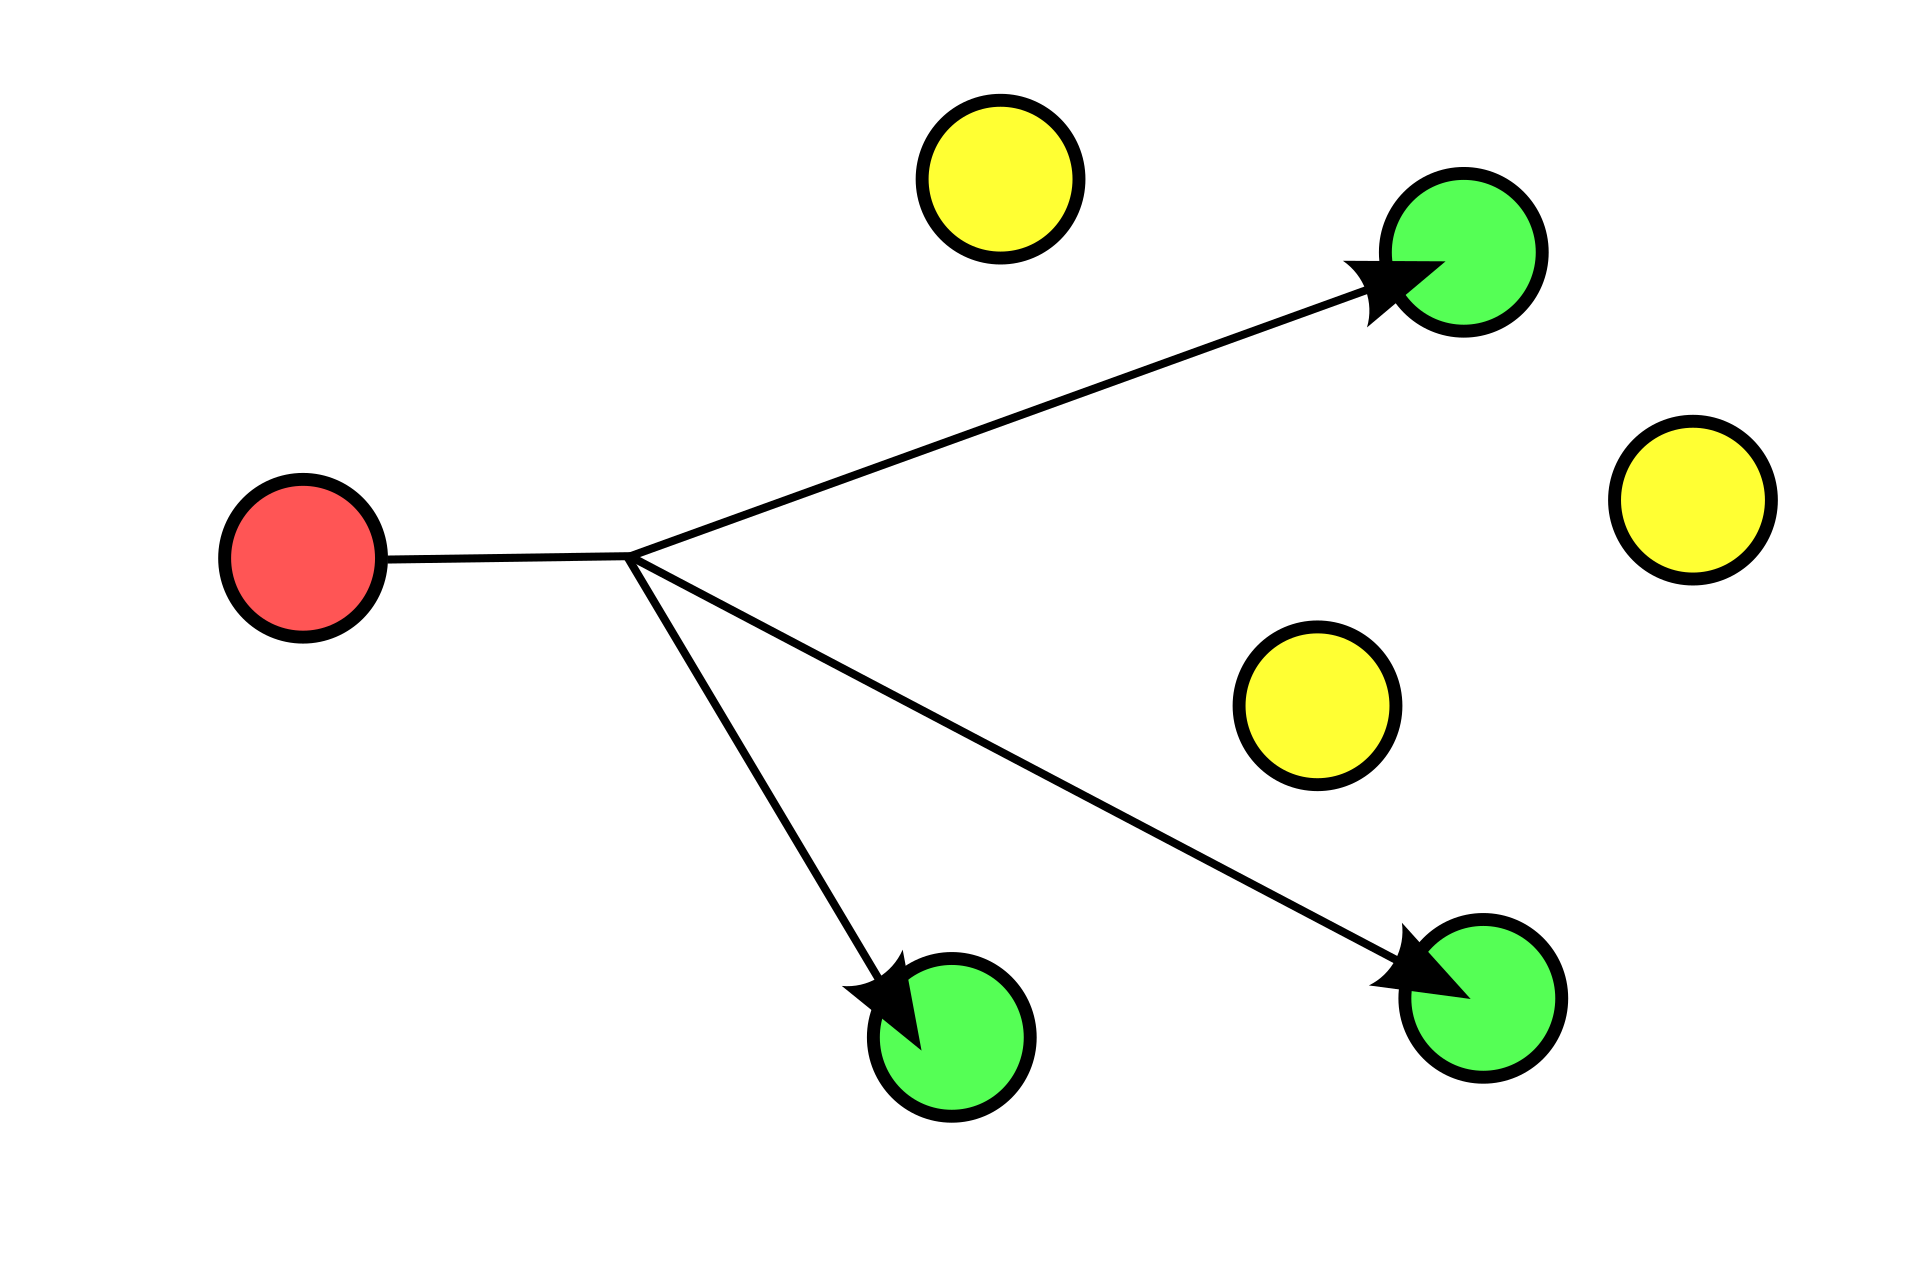
\includegraphics[width=\textwidth]{images/multicast.png}
   \caption[Multicast routing scheme]{Multicast routing}
   \label{fig:multicast}
   \end{minipage}
   \hfill
   \begin{minipage}{.4\textwidth}
   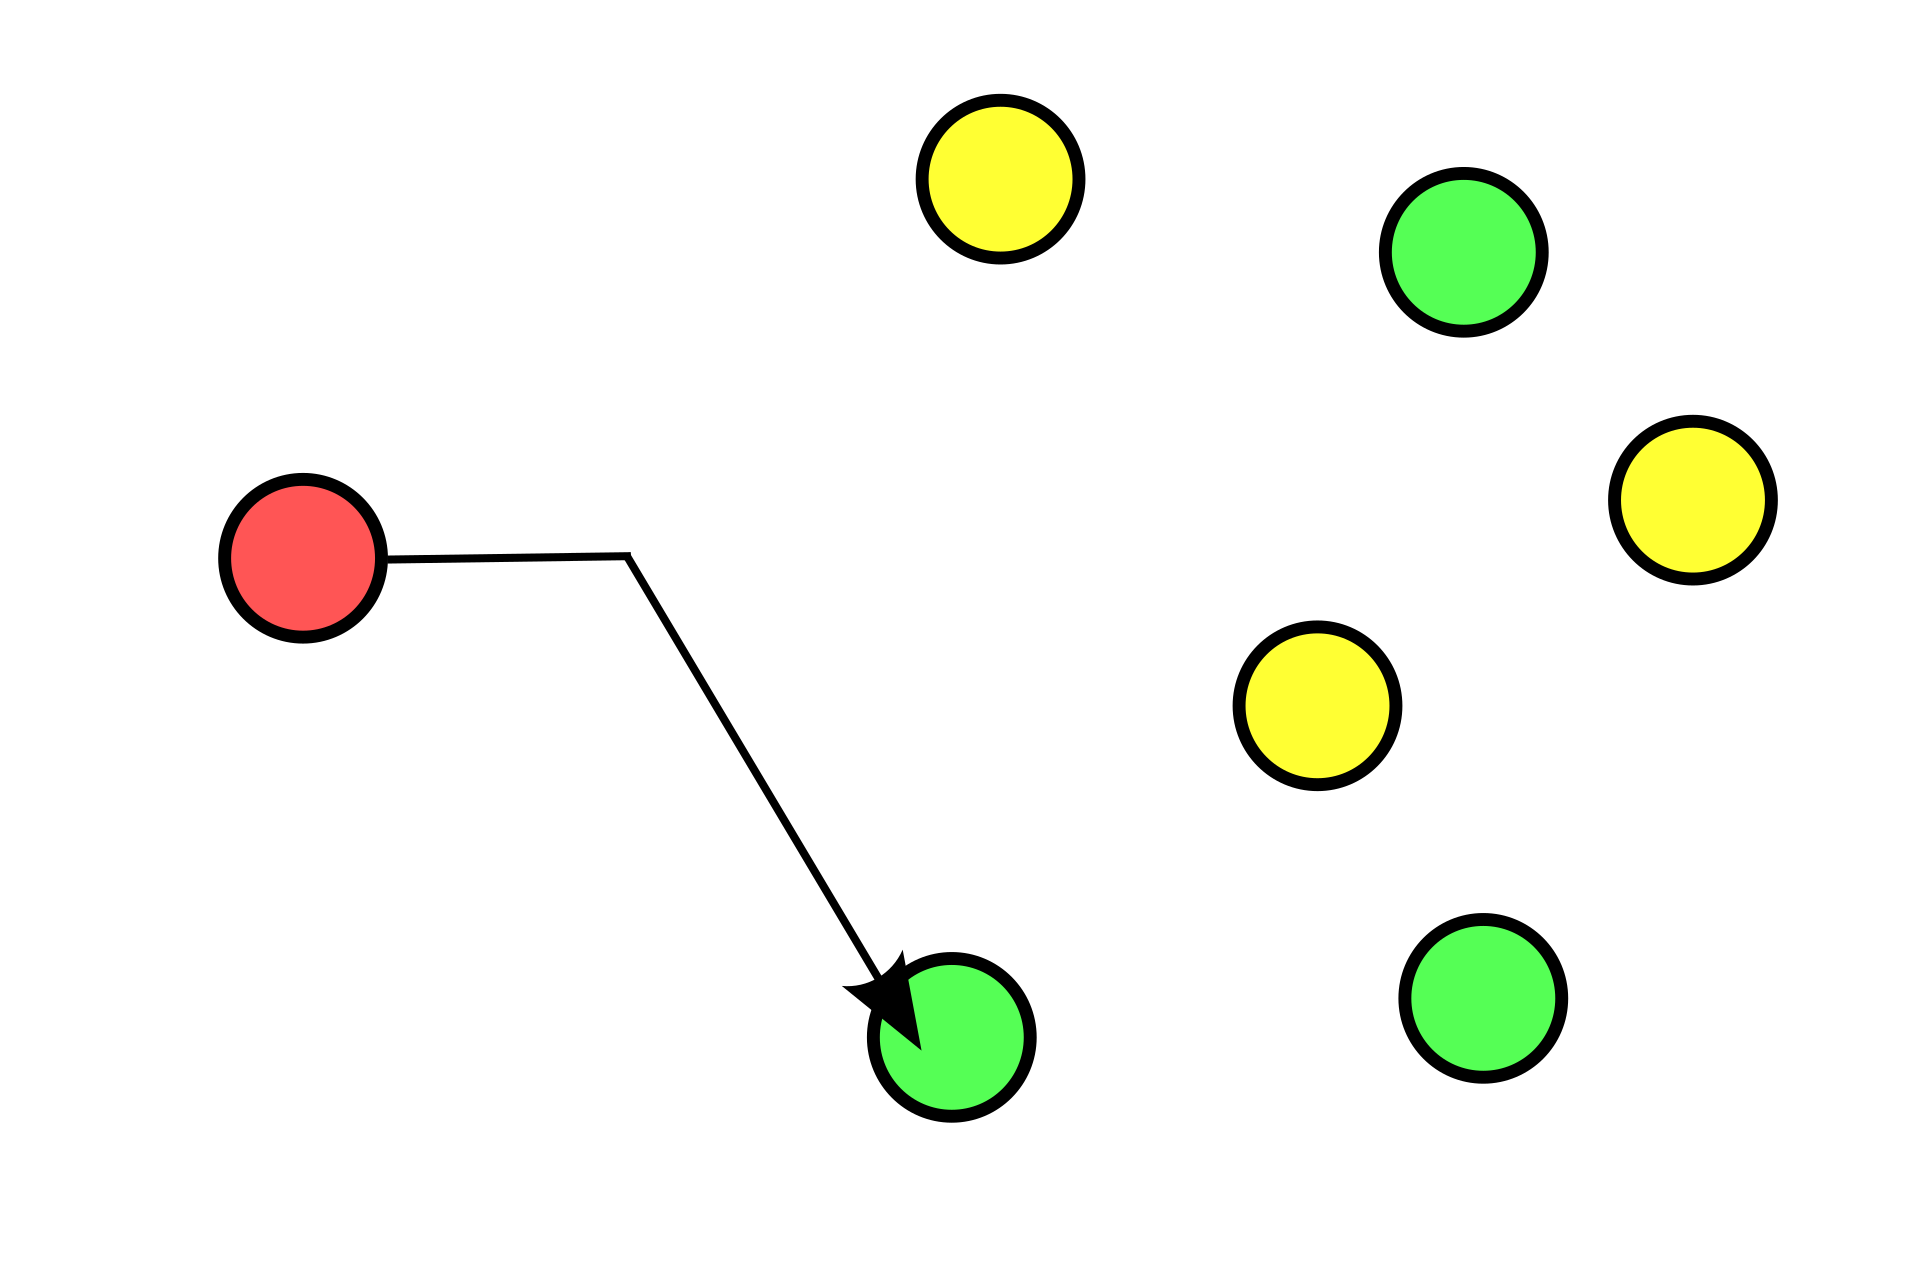
\includegraphics[width=\textwidth]{images/anycast.png}
   \caption[Anycast routing scheme]{Anycast routing}
   \label{fig:anycast}
   \end{minipage}
   \end{figure}
}

\mode<article>{
In this course we will only cover unicast and broadcast.
Multicast and anycast are only used in very specific networks.
}

\Section{Network models}
\label{sec:network-models}

\Paragraph{\acs{OSI} model}
\mode<article>{
      \index{network model!OSI model@\acs{OSI}}
The \acf{OSI} model  (see \vref{fig:network-models}) is a conceptual model that describes the universal standard of communication functions of a telecommunication system or computing system, without any regard to the system's underlying internal technology and specific protocol suites.
}

\Paragraph{\acs{TCP}/\acs{IP} model}
\mode<article>{
      \index{network model!TCP/IP model@\acs{TCP}/\acs{IP}}
      \index{network model!DoD@\acs{DOD}}
The \acs{TCP}/\acs{IP} model is also known as the DoD model because the development of the networking method was funded by the United States Department of Defense through \acs{DARPA}.
The \acl{IP} suite predates the \gls{OSI} model, a more comprehensive reference framework for general networking systems.
}

\Paragraph{hybrid model}
\mode<article>{
      \index{network model!hybrid}
\textcite[53]{comer}, \textcite[129]{kozierok}, \textcite[70]{tanenbaum}, and others use a hybrid, five-layer model, which I also prefer to use.
The upper layers (session, presentation, and application) are not important for a network engineer, nor are they clearly separated.
It is advisable to keep the bottom two layers separate. The data link layer comprises Ethernet switches, and it falls under the domain of network engineers, whereas the physical layer is the responsibility of network cabling technicicans.
}

\mode<article>{
\begin{figure}
\centering
\tikzstyle{box}=[
    minimum width=25mm,
    minimum height=8mm,
    font=\small\sffamily,
    text=black,
    node distance=8mm
]
\tikzstyle{upper}=[
    box,
    draw=spot4,
    fill=spot4!20
]
\tikzstyle{middle}=[
    box,
    draw=spot1,
    fill=spot1!20
]
\tikzstyle{lower}=[
    box,
    draw=spot2,
    fill=spot2!20
]

\begin{tikzpicture}

% OSI model
\node[upper]  (OSI7) [label=left:7.]               {application};
\node[upper]  (OSI6) [label=left:6.,below of=OSI7] {presentation};
\node[upper]  (OSI5) [label=left:5.,below of=OSI6] {session};
\node[middle] (OSI4) [label=left:4.,below of=OSI5] {transport};
\node[middle] (OSI3) [label=left:3.,below of=OSI4] {network};
\node[lower]  (OSI2) [label=left:2.,below of=OSI3] {data link};
\node[lower]  (OSI1) [label=left:1.,below of=OSI2] {physical};
\node         (OSI)  [below of=OSI1,node distance=12mm,minimum height=16mm]               {\small(\textsc{a}) OSI model};

% TCP/IP model
\node[upper]  (TCPIP4) [label=left:4.,right of=OSI6,%
                    node distance=35mm,minimum height=24mm]  {application};
\node[middle] (TCPIP3) [label=left:3.,below of=TCPIP4,
                    node distance=16mm]                      {transport};
\node[middle] (TCPIP2) [label=left:2.,below of=TCPIP3]       {internet};
\node[lower]  (TCPIP1) [label=left:1.,below of=TCPIP2,
                    node distance=12mm,minimum height=16mm]  {link};
\node         (TCPIP)  [below of=TCPIP1,node distance=16mm,minimum height=16mm]  {\small(\textsc{b}) TCP/IP model};

% hybrid model
\node[upper]  (hybrid5) [label=left:5.,right of=TCPIP4,
                    node distance=35mm,minimum height=24mm]  {application};
\node[middle] (hybrid4) [label=left:3.,below of=hybrid5,
                    node distance=16mm]                      {transport};
\node[middle] (hybrid3) [label=left:2.,below of=hybrid4]     {network};
\node[lower]  (hybrid2) [label=left:2.,below of=hybrid3]     {data link};
\node[lower]  (hybrid1) [label=left:1.,below of=hybrid2]     {physical};
\node         (hybrid)  [below of=hybrid1,node distance=12mm,minimum height=16mm]               {\small(\textsc{c}) hybrid model};
\end{tikzpicture}
\caption[The \acs{OSI}, \acs{TCP}/\acs{IP}, and hybrid networking models]{The three network models}
\label{fig:network-models}
\end{figure}
}

\slide{\tikzstyle{box}=[
    minimum width=25mm,
    minimum height=8mm,
    font=\small\sffamily,
    text=black,
    node distance=8mm
]
\tikzstyle{upper}=[
    box,
    draw=spot4,
    fill=spot4!20
]
\tikzstyle{middle}=[
    box,
    draw=spot1,
    fill=spot1!20
]
\tikzstyle{lower}=[
    box,
    draw=spot2,
    fill=spot2!20
]

\begin{tikzpicture}

% OSI model
\node[upper]  (OSI7) [label=left:7.]               {application};
\node[upper]  (OSI6) [label=left:6.,below of=OSI7] {presentation};
\node[upper]  (OSI5) [label=left:5.,below of=OSI6] {session};
\node[middle] (OSI4) [label=left:4.,below of=OSI5] {transport};
\node[middle] (OSI3) [label=left:3.,below of=OSI4] {network};
\node[lower]  (OSI2) [label=left:2.,below of=OSI3] {data link};
\node[lower]  (OSI1) [label=left:1.,below of=OSI2] {physical};
\node         (OSI)  [below of=OSI1,node distance=12mm,minimum height=16mm]               {\small(\textsc{a}) OSI model};

% TCP/IP model
\node[upper]  (TCPIP4) [label=left:4.,right of=OSI6,%
                    node distance=35mm,minimum height=24mm]  {application};
\node[middle] (TCPIP3) [label=left:3.,below of=TCPIP4,
                    node distance=16mm]                      {transport};
\node[middle] (TCPIP2) [label=left:2.,below of=TCPIP3]       {internet};
\node[lower]  (TCPIP1) [label=left:1.,below of=TCPIP2,
                    node distance=12mm,minimum height=16mm]  {link};
\node         (TCPIP)  [below of=TCPIP1,node distance=16mm,minimum height=16mm]  {\small(\textsc{b}) TCP/IP model};

% hybrid model
\node[upper]  (hybrid5) [label=left:5.,right of=TCPIP4,
                    node distance=35mm,minimum height=24mm]  {application};
\node[middle] (hybrid4) [label=left:3.,below of=hybrid5,
                    node distance=16mm]                      {transport};
\node[middle] (hybrid3) [label=left:2.,below of=hybrid4]     {network};
\node[lower]  (hybrid2) [label=left:2.,below of=hybrid3]     {data link};
\node[lower]  (hybrid1) [label=left:1.,below of=hybrid2]     {physical};
\node         (hybrid)  [below of=hybrid1,node distance=12mm,minimum height=16mm]               {\small(\textsc{c}) hybrid model};
\end{tikzpicture}}


\Section{Network communication}
\label{sec:network-communication}

\Paragraph{How to reach the server?}
\mode<article>{
You will need the \acs{IP} address of the computer you want to communicate with.
We can get this address using the \acl{DNS} (see \vref{chap:applications}) and we can use a search engine to find the domain names of the websites we want to access.
}

\Paragraph{Which application is the data for?}
\mode<article>{
We will use \emph{port numbers} (see \vref{chap:transport-layer}) to indicate which application the data is for.
}

\Paragraph{How to send a lot of data?}
\mode<article>{
   \acs{MTU}
   \index{fragmentation}
Not all protocols allow us to send the same amount of data.
For example, Ethernet limits the packet size to 1522~bytes while \gls{ATM} had a limit of 53~bytes per packet.
This means that, depending on the protocol in use, we will have to \emph{fragment} our data in smaller pieces and the destination will need to piece back these pieces together.
}

\Paragraph{What if something goes wrong?}
\mode<article>{
Data can get corrupted or lost in transit.
Different protocols will deal differently with these issues.
Ethernet (\vref{chap:ethernet}) only has an error detection code while \acf{TCP} (\vref{sec:tcp}) garanties correct delivery of data.
}

\Section{Encapsulation}
\label{sec:encapsulation}

\mode<article>{
\Vref{fig:encapsulation} shows the five layers of the hybrid model and the different headers (and trailer) which get added by each layer.
When data gets send from the host on the left to the host on the right, the application passes the data to the operating system's kernel to be sent on the network.
For each layer of the protocol stack a header gets added so that the corresponding layer on the receiver's side knows what the data is for.
That is, the transport layer on the sender's side communicates with the transport layer on the receiver's side and the network layer on the sender's side communicates with the corresponding layer on the receiver's side.

\begin{figure}
\centering
\tikzstyle{layer}=[
    minimum width=25mm,
    minimum height=8mm,
    inner sep=0mm,
    font=\small\sffamily,
    text=black,
    node distance=12mm,
    draw=spot1,
    fill=spot1!20
]
\tikzstyle{arrow}=[->,>=stealth',semithick]
\tikzstyle{red arrow}=[arrow,very thick,spot2]
\tikzstyle{packet data}=[
    rectangle,
    draw=spot4,
    fill=spot4!20,
    text=black,
    thin,
    minimum height=8mm,
    minimum width=12mm,
    inner sep=0mm
]
\tikzstyle{packet header}=[
    rectangle,
    draw=spot5,
    fill=spot5!20,
    text=black,
    thin,
    node distance=8mm,
    minimum size=8mm,
    inner sep=0mm
]
\begin{tikzpicture}

% two network stacks
\node[layer] (a1)               {application};
\node[layer] (t1) [below of=a1] {transport};
\node[layer] (n1) [below of=t1] {network};
\node[layer] (d1) [below of=n1] {data link};
\node[layer] (p1) [below of=d1] {physical};

\node[layer] (a2) [right of=a1,node distance=90mm]  {application};
\node[layer] (t2) [below of=a2]                     {transport};
\node[layer] (n2) [below of=t2]                     {network};
\node[layer] (d2) [below of=n2]                     {data link};
\node[layer] (p2) [below of=d2]                     {physical};

\draw[arrow] (a1) -- (t1);
\draw[arrow] (t1) -- (n1);
\draw[arrow] (n1) -- (d1);
\draw[arrow] (d1) -- (p1);

\draw[arrow] (t2) -- (a2);
\draw[arrow] (n2) -- (t2);
\draw[arrow] (d2) -- (n2);
\draw[arrow] (p2) -- (d2);

\draw[red arrow] (a1) to node[packet data] {data} (a2);
\draw[red arrow] (t1) to node[packet data] (dt) {data}
                         node[packet header,left of=dt,node distance=10mm] {t}
                         (t2);
\draw[red arrow] (n1) to node[packet data] (dn) {data}
                         node[packet header,left of=dn,node distance=10mm] (hn1) {t} node[packet header,left of=dn,node distance=18mm] (hn2) {n}
                         (n2);
\draw[red arrow] (d1) to node[packet data] (dd) {data}
                         node[packet header,left of=dd,node distance=10mm] (hd1) {t} node[packet header,left of=dd,node distance=18mm] (hd2) {n} node[packet header,left of=dd,node distance=26mm] (hd3) {d} node[packet header,right of=dd,node distance=10mm] (td) {d}
                         (d2);
\end{tikzpicture}
\caption[Encapsulation and decapsulation of packets]{%
Data encapsulation at the source and decapsulation at the destination.
Each layer adds its own header, but the data link layer also adds a trailer.
}
\label{fig:encapsulation}
\end{figure}

The data combined with the transport layer header is called a \emph{segment};
a segment and the network layer header is called a \emph{packet};
a packet and the data link header and trailer is called a \emph{frame}.
}
\slide{\scalebox{.7}{\tikzstyle{layer}=[
    minimum width=25mm,
    minimum height=8mm,
    inner sep=0mm,
    font=\small\sffamily,
    text=black,
    node distance=12mm,
    draw=spot1,
    fill=spot1!20
]
\tikzstyle{arrow}=[->,>=stealth',semithick]
\tikzstyle{red arrow}=[arrow,very thick,spot2]
\tikzstyle{packet data}=[
    rectangle,
    draw=spot4,
    fill=spot4!20,
    text=black,
    thin,
    minimum height=8mm,
    minimum width=12mm,
    inner sep=0mm
]
\tikzstyle{packet header}=[
    rectangle,
    draw=spot5,
    fill=spot5!20,
    text=black,
    thin,
    node distance=8mm,
    minimum size=8mm,
    inner sep=0mm
]
\begin{tikzpicture}

% two network stacks
\node[layer] (a1)               {application};
\node[layer] (t1) [below of=a1] {transport};
\node[layer] (n1) [below of=t1] {network};
\node[layer] (d1) [below of=n1] {data link};
\node[layer] (p1) [below of=d1] {physical};

\node[layer] (a2) [right of=a1,node distance=90mm]  {application};
\node[layer] (t2) [below of=a2]                     {transport};
\node[layer] (n2) [below of=t2]                     {network};
\node[layer] (d2) [below of=n2]                     {data link};
\node[layer] (p2) [below of=d2]                     {physical};

\draw[arrow] (a1) -- (t1);
\draw[arrow] (t1) -- (n1);
\draw[arrow] (n1) -- (d1);
\draw[arrow] (d1) -- (p1);

\draw[arrow] (t2) -- (a2);
\draw[arrow] (n2) -- (t2);
\draw[arrow] (d2) -- (n2);
\draw[arrow] (p2) -- (d2);

\draw[red arrow] (a1) to node[packet data] {data} (a2);
\draw[red arrow] (t1) to node[packet data] (dt) {data}
                         node[packet header,left of=dt,node distance=10mm] {t}
                         (t2);
\draw[red arrow] (n1) to node[packet data] (dn) {data}
                         node[packet header,left of=dn,node distance=10mm] (hn1) {t} node[packet header,left of=dn,node distance=18mm] (hn2) {n}
                         (n2);
\draw[red arrow] (d1) to node[packet data] (dd) {data}
                         node[packet header,left of=dd,node distance=10mm] (hd1) {t} node[packet header,left of=dd,node distance=18mm] (hd2) {n} node[packet header,left of=dd,node distance=26mm] (hd3) {d} node[packet header,right of=dd,node distance=10mm] (td) {d}
                         (d2);
\end{tikzpicture}}}

\Paragraph{port numbers}
\mode<article>{
The segment header at the transport layer adds port numbers to indicate which application the data is destined for and which application the data came from.
}

\Paragraph{\acs{IP} addresses}
\mode<article>{
The packet header at the network layer adds \acs{IP} addresses indicating which host the data is destined for and which host it came from.
}

\Paragraph{\acf{DNS}}
\mode<article>{
\acs{DNS} is used to find the \acs{IP} address of the destination host.
See \vref{chap:applications} for more details.
}

\Paragraph{\acs{MAC} addresses}
\mode<article>{
\acs{MAC} addresses are added to the frame header at the data link layer.
They are used to deliver the frame on the local network.
See \vref{chap:ethernet} for further details.
}

\Paragraph{\acf{ARP}}
\mode<article>{
   \iacs{ARP}
The \acl{ARP} is a communication protocol used for discovering the data link layer address, such as a \acs{MAC} address, associated with a given network layer address, typically an \acs{IP} version~4 address.

Two computers in an office (host~$A$ and host~$B$) are connected to each other in a local-area network by Ethernet cables and network switches, with no intervening gateways or routers.
Host~$A$ has a packet to send to host~$B$.
Through \acs{DNS}, it determines that host~$B$ has the \acs{IP} address 203.0.113.55.

To send the message, it also requires host~$B$'s \acs{MAC} address.
First, host~$A$ uses a cached \acs{ARP} table to look up 203.0.113.55 for any existing records of host~$B$'s \acs{MAC} address (00eb.\-24b2.\-05ac).
If the \acs{MAC} address is found, it sends an Ethernet frame containing the \acs{IP} packet onto the link with the destination address 00eb.\-24b2.\-05ac.
If the cache did not produce a result for 203.0.113.55, host~$A$ has to send a broadcast \acs{ARP} request message (with the destination \acs{MAC} address of ffff.\-ffff.\-ffff), which is accepted by all computers on the local network, requesting an answer for 203.0.113.55.

Host~$B$ responds with an \acs{ARP} response message containing its \acs{MAC} and \acs{IP} addresses.
As part of fielding the request, host~$B$ may insert an entry for host~$A$ into its \acs{ARP} table for future use.
Host~$A$ receives and caches the response information in its \acs{ARP} table and can now send the packet.

The above example assumes both computers are located on the same local network.
Host~$A$ needs to determine this is the case by \abbr{AND}'ing%
\footnote{\abbr{AND} is a binary operator used in boolean algebra. It returns a 1 if both its inputs are 1 and returns a 0 in all other cases.}
both its own \acs{IP} address and the \acs{IP} address of the second computer with its own \emph{subnet mask}.%
   \index{subnet mask}
If both results match, both computers are located in the same network; otherwise the second computer is located in a remote network and we need to send the frame to the \emph{default gateway}%
\footnote{Or to a different \emph{gateway}, depending on the routing table. See \vref{sec:routing} for more details.}
instead.%
   \index{default gateway}

In this case, host~$A$ sends an \acs{ARP} request -- assuming there is no valid entry in its cache -- for the \acs{MAC} address of the default gateway.
When the default gateway receives this frame, it verifies the frame is addressed to its \acs{MAC} address but the destination \acs{IP} address is none an \acs{IP} address owned by the router so it must forward the packet to further along to the destination.
See \vref{sec:routing} on how routers work.

\Vref{fig:data-flow} shows a topology with two routers between the source and the destination.
Each router, when sending the frame forward, must do an \acs{ARP} lookup to generate a new frame header as \acs{MAC} addresses are local to a given network segment.
It is the only layer that gets stripped and regenerated at each router hop.
The network and transport layers are host-to-host.


\begin{figure}
\centering
\tikzstyle{enode}=[
    draw=nodelinecolor,thick,
    fill=nodefillcolor,
    minimum size=10mm,
    inner sep=0mm,
    text=nodelinecolor
]
\tikzstyle{nnode}=[
    circle,
    draw=nodelinecolor,thick,
    fill=nodefillcolor,
    minimum size=10mm,
    inner sep=0mm,
    text=nodelinecolor
]
\tikzstyle{arrow}=[->,>=stealth',semithick]
\tikzstyle{double arrow}=[<->,>=stealth',very thick,spot2,dashed]
%\tikzstyle{layer}=[
%    draw=nodelinecolor,thick,
%    fill=nodefillcolor,
%    minimum height=8mm,
%    minimum width=20mm,
%    inner sep=0mm,
%    text=nodelinecolor,
%    node distance=12mm
%]
\tikzstyle{layer}=[
    minimum width=20mm,
    minimum height=8mm,
    inner sep=0mm,
    font=\small\sffamily,
    text=black,
    node distance=12mm,
    draw=spot1,
    fill=spot1!20
]

\begin{tikzpicture}[node distance=18mm]

% network topology
\node at (45mm,12mm) {\bfseries network topology};
\node[enode] (A)                {\footnotesize host A};
\node[nnode] (R1) [node distance=30mm,right of=A]  {\footnotesize router};
\node[nnode] (R2) [node distance=30mm,right of=R1] {\footnotesize router};
\node[enode] (B)  [node distance=30mm,right of=R2] {\footnotesize host B};
\draw[arrow] (A) -- (R1);
\draw[arrow] (R1)-- (R2);
\draw[arrow] (R2)-- (B);

% data flow
\node at (45mm,-18mm) {\bfseries data flow};
\node[layer] (AA) [below of=A,node distance=30mm] {\small application};
\node[layer] (AT) [below of=AA]                   {\small transport};
\node[layer] (AN) [below of=AT]                   {\small network};
\node[layer] (AD) [below of=AN]                   {\small data link};
\draw[arrow] (AA) -- (AT);
\draw[arrow] (AT) -- (AN);
\draw[arrow] (AN) -- (AD);

\node[layer] (BA) [below of=B,node distance=30mm] {\small application};
\node[layer] (BT) [below of=BA]                   {\small transport};
\node[layer] (BN) [below of=BT]                   {\small network};
\node[layer] (BD) [below of=BN]                   {\small data link};
\draw[arrow] (BT) -- (BA);
\draw[arrow] (BN) -- (BT);
\draw[arrow] (BD) -- (BN);

\draw[double arrow] (AA) to node[auto,color=black] {\footnotesize process-to-process} (BA);
\draw[double arrow] (AT) to node[auto,color=black] {\footnotesize host-to-host} (BT);

\node[layer] (R1N) [node distance=30mm,right of=AN]  {\small network};
\node[layer] (R2N) [node distance=30mm,right of=R1N] {\small network};
\node[layer] (R1D) [node distance=30mm,right of=AD]  {\small data link};
\node[layer] (R2D) [node distance=30mm,right of=R1D] {\small data link};

\draw[arrow] ($(R1N.south)+(.2,0)$) -- ($(R1D.north)+(.2,0)$);
\draw[arrow] ($(R1D.north)-(.2,0)$) -- ($(R1N.south)-(.2,0)$);
\draw[arrow] ($(R2N.south)+(.2,0)$) -- ($(R2D.north)+(.2,0)$);
\draw[arrow] ($(R2D.north)-(.2,0)$) -- ($(R2N.south)-(.2,0)$);

\draw[arrow] (AD)                   -- ($(AD.south) -(0 , .5)$) -| ($(R1D.south)-(.2,0)$);
\draw[arrow] ($(R1D.south)+(.2,0)$) -- ($(R1D.south)+(.2,-.5)$) -| ($(R2D.south)-(.2,0)$);
\draw[arrow] ($(R2D.south)+(.2,0)$) -- ($(R2D.south)+(.2,-.5)$) -| (BD.south);

\end{tikzpicture}
\caption{Encapsulation and data flow in the network}
\label{fig:data-flow}
\end{figure}


\Cref{fig:data-flow} is a bit misleading in this way.
Although the routers check the \acs{IP} addresses of the network layer header, the header does not change significantly.
See \vref{sec:nat} for an example of a router that changes the \acs{IP} addresses in the header.
}

\Section{Network icons}
\label{sec:network-icons}

\mode<article>{
\Vref{fig:icons} shows the three basic network icons used most often in network drawings.
Many different variants exist for these icons, depending on taste or function (e.g.~a core switch versus an access switch).
There are more icons available for devices such as wireless \acs{LAN} controllers, acccess points, load balancers, and many more.
\begin{figure}
   \centering
   \begin{subfigure}[b]{18mm}
   
\includegraphics[width=\textwidth]{images/router.jpg}
   \caption{router}
   \label{fig:icon-router}
   \end{subfigure}
   \qquad
   \begin{subfigure}[b]{18mm}
   
\includegraphics[width=\textwidth]{images/switch.png}
   \caption{switch}
   \label{fig:icon-switch}
   \end{subfigure}
   \qquad
   \begin{subfigure}[b]{18mm}
   
\includegraphics[width=\textwidth]{images/firewall.png}
   \caption{firewall}
   \label{fig:icon-firewall}
   \end{subfigure}
   \caption{Network icons for a router, a switch, and a firewall}
   \label{fig:icons}
\end{figure}
}
\slide{
   
\includegraphics[width=.1\textwidth]{images/router.jpg}\qquad%
   
\includegraphics[width=.1\textwidth]{images/switch.png}\qquad%
   
\includegraphics[width=.1\textwidth]{images/firewall.png}
}